%%%%%%%%%%%%%%%%%%%%%%%%%%%%%%%%%%%%%%%%%%%%%%%%%%%%%%%%%%%%%
%% Begin exercise %%
%%%%%%%%%%%%%%%%%%%%%%%%%%%%%%%%%%%%%%%%%%%%%%%%%%%%%%%%%%%%%
\ex{High-frequency magnetics: materials and core loss}

%%%%%%%%%%%%%%%%%%%%%%%%%%%%%%%%%%%%%%%%%%%%%%%%%%%%%%%%%%%%%
%% Task 1 %%
%%%%%%%%%%%%%%%%%%%%%%%%%%%%%%%%%%%%%%%%%%%%%%%%%%%%%%%%%%%%%

\task{Saturation or loss limit}

A MnZn power ferrite is described at $\SI{100}{\celsius}$ by $P_\mathrm{v}=\SI{80}{\kilo\watt\per\cubic\metre}$ at $\SI{100}{\kilo\hertz}$ and $\SI{100}{\milli\tesla}$ (sinusoidal flux), $\alpha=1.4$, $\beta=2.5$ and $B_\mathrm{sat}=\SI{370}{\milli\tesla}$. The allowed loss density is $\SI{300}{\kilo\watt\per\cubic\metre}$.

\subtask{Above which frequency $f_\mathrm{x}$ is the flux density limited by core loss rather than by saturation?}

\begin{solutionblock}
	At $B_\mathrm{sat}$ and $\SI{100}{\kilo\hertz}$ the loss density would be $80\cdot3.7^{2.5}\,\si{\kilo\watt\per\cubic\metre}=\SI{2107}{\kilo\watt\per\cubic\metre}$. It falls to the allowed value at
	\begin{equation}
		f_\mathrm{x}=\SI{100}{\kilo\hertz}\cdot\left(\frac{300}{2107}\right)^{1/1.4}=\SI{24.9}{\kilo\hertz}.
	\end{equation}
	Every design above a few tens of kHz is loss-limited.
\end{solutionblock}

\subtask{Calculate the allowed flux density $\hat{B}$ and the performance factor $\hat{B}f$ at $\SI{100}{\kilo\hertz}$ and $\SI{400}{\kilo\hertz}$. How does $\hat{B}f$ scale with frequency?}

\begin{solutionblock}
	\begin{equation}
		\hat{B}=\SI{100}{\milli\tesla}\cdot\left(\frac{300}{80}\right)^{1/2.5}\left(\frac{f}{\SI{100}{\kilo\hertz}}\right)^{-1.4/2.5}
	\end{equation}
	gives $\SI{170}{\milli\tesla}$ at $\SI{100}{\kilo\hertz}$ and $\SI{78}{\milli\tesla}$ at $\SI{400}{\kilo\hertz}$, i.e.\ $\hat{B}f=17.0$ and $\SI{31.2}{\milli\tesla\cdot\mega\hertz}$. In the loss-limited range $\hat{B}f\propto f^{1-\alpha/\beta}=f^{0.44}$: four times the frequency gives only 1.84 times the VA of the core.
\end{solutionblock}

\subtask{Compare with the NiZn ferrite Fair-Rite 67 at $\SI{10}{\mega\hertz}$ ($P_\mathrm{v}=k\hat{B}^{\beta}$ with $k=2.09$, $\beta=2.08$, $P_\mathrm{v}$ in $\si{\milli\watt\per\cubic\centi\metre}$, $\hat{B}$ in mT) at the same loss density.}

\begin{solutionblock}
	$\SI{300}{\kilo\watt\per\cubic\metre}=\SI{300}{\milli\watt\per\cubic\centi\metre}$: $\hat{B}=(300/2.09)^{1/2.08}=\SI{10.9}{\milli\tesla}$, $\hat{B}f=\SI{109}{\milli\tesla\cdot\mega\hertz}$. Going from $\SI{400}{\kilo\hertz}$ to $\SI{10}{\mega\hertz}$ increases the VA per core volume by a factor of 3.5, not 25.
\end{solutionblock}

%%%%%%%%%%%%%%%%%%%%%%%%%%%%%%%%%%%%%%%%%%%%%%%%%%%%%%%%%%%%%
%% Task 2 %%
%%%%%%%%%%%%%%%%%%%%%%%%%%%%%%%%%%%%%%%%%%%%%%%%%%%%%%%%%%%%%

\task{Performance factor in the HF range}

Hanson et al.\ (IEEE TPEL, 2016) measured Fair-Rite 67 ($\mu_\mathrm{r}=40$) and fitted $P_\mathrm{v}=k\hat{B}^{\beta}$ ($P_\mathrm{v}$ in $\si{\milli\watt\per\cubic\centi\metre}$, $\hat{B}$ in mT) at each frequency:

\begin{table}[ht]
	\centering
	\begin{tabular}{|l|c|c|c|c|}
		\hline
		$f$ in MHz & 2    & 5    & 10   & 20    \\
		\hline
		$k$        & 0.10 & 0.69 & 2.09 & 10.95 \\
		$\beta$    & 2.44 & 2.20 & 2.08 & 1.99  \\
		\hline
	\end{tabular}
	\caption{Steinmetz parameters of Fair-Rite 67}
	\label{tab:ex06_fr67}
\end{table}

\subtask{Calculate $\hat{B}$ at $\SI{500}{\milli\watt\per\cubic\centi\metre}$ and the performance factors $\hat{B}f$, $\hat{B}f^{3/4}$ and $\hat{B}f^{1/2}$ for each frequency.}

\begin{solutionblock}
	$\hat{B}=(500/k)^{1/\beta}$:
	\begin{solutiontable}[ht]
		\centering
		\begin{tabular}{|l|c|c|c|c|}
			\hline
			$f$ in MHz                                      & 2    & 5    & 10    & 20    \\
			\hline
			$\hat{B}$ in mT                                 & 32.8 & 20.0 & 13.9  & 6.8   \\
			$\hat{B}f$ in mT$\cdot$MHz                       & 65.6 & 99.8 & 139.2 & 136.5 \\
			$\hat{B}f^{3/4}$ in mT$\cdot$MHz$^{3/4}$         & 55.2 & 66.7 & 78.3  & 64.5  \\
			$\hat{B}f^{1/2}$ in mT$\cdot$MHz$^{1/2}$         & 46.4 & 44.6 & 44.0  & 30.5  \\
			\hline
		\end{tabular}
	\end{solutiontable}
\end{solutionblock}

\subtask{Which frequency gives the smallest core (at this loss density) for (a) a winding without skin and proximity effect, (b) single-layer windings, (c) a winding with fixed strand or layer thickness?}

\begin{solutionblock}
	(a) $\hat{B}f$: 10 to $\SI{20}{\mega\hertz}$, more than twice the value at $\SI{2}{\mega\hertz}$. (b) $\hat{B}f^{3/4}$: $\SI{10}{\mega\hertz}$, 1.42 times the value at $\SI{2}{\mega\hertz}$. (c) $\hat{B}f^{1/2}$: no gain above $\SI{2}{\mega\hertz}$; litz wire with a given strand diameter does not profit from a higher frequency.
\end{solutionblock}

\subtask{Calculate the loss density at $\hat{B}=\SI{10}{\milli\tesla}$ and estimate the frequency exponent $\alpha$ between 2 and $\SI{10}{\mega\hertz}$ and between 10 and $\SI{20}{\mega\hertz}$. Explain the course of $\hat{B}f$.}

\begin{solutionblock}
	$P_\mathrm{v}(\SI{10}{\milli\tesla})=27.5$, 109, 251 and $\SI{1070}{\milli\watt\per\cubic\centi\metre}$ at 2, 5, 10 and $\SI{20}{\mega\hertz}$:
	\begin{equation}
		\alpha_{2\ldots10}=\frac{\ln(251/27.5)}{\ln5}=1.37,\qquad\alpha_{10\ldots20}=\frac{\ln(1070/251)}{\ln2}=2.09.
	\end{equation}
	Below $\SI{10}{\mega\hertz}$ $\alpha<\beta$ and $\hat{B}f$ rises; above, $\alpha$ exceeds $\beta\approx2.0$ and $\hat{B}f$ stops rising. The material has reached its frequency limit.
\end{solutionblock}

%%%%%%%%%%%%%%%%%%%%%%%%%%%%%%%%%%%%%%%%%%%%%%%%%%%%%%%%%%%%%
%% Task 3 %%
%%%%%%%%%%%%%%%%%%%%%%%%%%%%%%%%%%%%%%%%%%%%%%%%%%%%%%%%%%%%%

\task{Planar transformer of an LLC DC transformer}

The transformer of brief B2 is driven by a full bridge with a square-wave voltage of $\pm\SI{48}{\volt}$ at $\SI{1}{\mega\hertz}$ (\autoref{fig:ex06_waveforms}a). Turns ratio 4:1, planar core with $A_\mathrm{e}=\SI{40}{\square\milli\metre}$ and $V_\mathrm{e}=\SI{1.0}{\cubic\centi\metre}$. Core material at $\SI{1}{\mega\hertz}$ and $\SI{100}{\celsius}$: $P_\mathrm{v}=\SI{150}{\kilo\watt\per\cubic\metre}$ at $\SI{50}{\milli\tesla}$ (sinusoidal), $\alpha=1.5$, $\beta=2.5$. With $N_\mathrm{p}=4$ the winding loss is $\SI{0.25}{\watt}$; it scales with $N_\mathrm{p}^2$, because the windings always fill the window. Hint: $\int_0^{2\pi}|\cos\theta|^{1.5}\,\mathrm{d}\theta=3.496$.

%%%%%%%%%%%%%%%%%%%%%%%%%%%%%%%%%%%%%%%%%%%%%%%%%%%%%%%%%%%%%%%%%%%%%%%%%%
% Voltage and flux waveforms of the transformer (Task 3) and the inductor (Task 4), Exercise 06
%%%%%%%%%%%%%%%%%%%%%%%%%%%%%%%%%%%%%%%%%%%%%%%%%%%%%%%%%%%%%%%%%%%%%%%%%%

\begin{figure}[htb]
	\begin{center}
		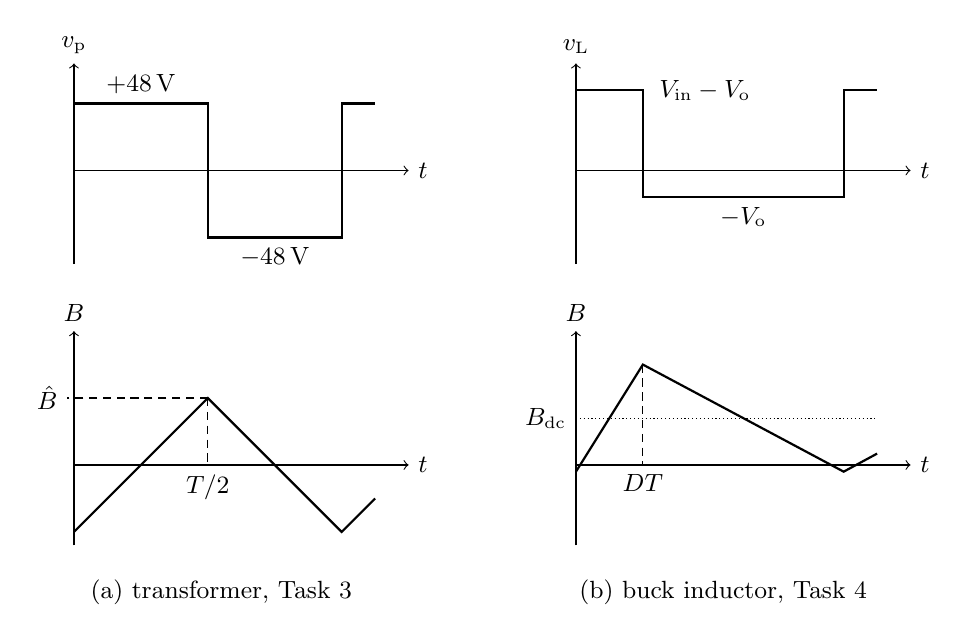
\begin{tikzpicture}[scale=0.85, every node/.style={font=\small}]
			% (a) transformer: square-wave voltage, triangular flux
			\draw[->] (0,0) -- (5.0,0) node[right]{$t$};
			\draw[->] (0,-1.4) -- (0,1.6) node[above]{$v_\mathrm{p}$};
			\draw[thick] (0,1) -- (2,1) -- (2,-1) -- (4,-1) -- (4,1) -- (4.5,1);
			\node[anchor=south] at (1,1) {$+48$\,V};
			\node[anchor=north] at (3,-1) {$-48$\,V};
			\draw[->] (0,-4.4) -- (5.0,-4.4) node[right]{$t$};
			\draw[->] (0,-5.6) -- (0,-2.4) node[above]{$B$};
			\draw[thick] (0,-5.4) -- (2,-3.4) -- (4,-5.4) -- (4.5,-4.9);
			\draw[densely dashed] (2,-3.4) -- (-0.1,-3.4) node[left]{$\hat{B}$};
			\draw[densely dashed] (2,-3.4) -- (2,-4.4) node[below]{$T/2$};
			\node at (2.2,-6.3) {(a) transformer, Task 3};
			% (b) buck inductor: asymmetric voltage, flux with DC component
			\begin{scope}[xshift=7.5cm]
				\draw[->] (0,0) -- (5.0,0) node[right]{$t$};
				\draw[->] (0,-1.4) -- (0,1.6) node[above]{$v_\mathrm{L}$};
				\draw[thick] (0,1.2) -- (1,1.2) -- (1,-0.4) -- (4,-0.4) -- (4,1.2) -- (4.5,1.2);
				\node[anchor=west] at (1.1,1.2) {$V_\mathrm{in}-V_\mathrm{o}$};
				\node[anchor=north] at (2.5,-0.4) {$-V_\mathrm{o}$};
				\draw[->] (0,-4.4) -- (5.0,-4.4) node[right]{$t$};
				\draw[->] (0,-5.6) -- (0,-2.4) node[above]{$B$};
				\draw[thick] (0,-4.5) -- (1,-2.9) -- (4,-4.5) -- (4.5,-4.23);
				\draw[densely dotted] (0,-3.7) -- (4.5,-3.7);
				\node[anchor=east] at (0,-3.7) {$B_\mathrm{dc}$};
				\draw[densely dashed] (1,-2.9) -- (1,-4.4) node[below]{$DT$};
				\node at (2.2,-6.3) {(b) buck inductor, Task 4};
			\end{scope}
		\end{tikzpicture}
	\end{center}
	\caption{Voltage and flux density of the transformer of Task 6.3 and of the inductor of Task 6.4 (not to scale)}
	\label{fig:ex06_waveforms}
\end{figure}


\subtask{Calculate $\hat{B}$ for $N_\mathrm{p}=4$ and $N_\mathrm{p}=8$.}

\begin{solutionblock}
	The flux changes by $\Delta B=2\hat{B}$ during half a period:
	\begin{equation}
		\hat{B}=\frac{V}{4fN_\mathrm{p}A_\mathrm{e}}=\frac{\SI{48}{\volt}}{4\cdot\SI{1}{\mega\hertz}\cdot N_\mathrm{p}\cdot\SI{40}{\square\milli\metre}},
	\end{equation}
	$\SI{75}{\milli\tesla}$ for $N_\mathrm{p}=4$ and $\SI{37.5}{\milli\tesla}$ for $N_\mathrm{p}=8$.
\end{solutionblock}

\subtask{Calculate the core loss with the iGSE.}

\begin{solutionblock}
	\begin{equation}
		k_\mathrm{i}=\frac{k}{(2\pi)^{\alpha-1}\,2^{\beta-\alpha}\int_0^{2\pi}|\cos\theta|^{\alpha}\,\mathrm{d}\theta}=\frac{k}{2.507\cdot2\cdot3.496}=0.0571\,k.
	\end{equation}
	For the symmetric triangle ($D=0.5$, $\Delta B=2\hat{B}$):
	\begin{equation}
		P_\mathrm{v}=k_\mathrm{i}(2\hat{B})^{\beta}f^{\alpha}\left(0.5^{-0.5}+0.5^{-0.5}\right)=0.0571\cdot5.657\cdot2.828\,kf^{\alpha}\hat{B}^{\beta}=0.913\,kf^{\alpha}\hat{B}^{\beta}.
	\end{equation}
	With $kf^{\alpha}\hat{B}^{\beta}=\SI{150}{\kilo\watt\per\cubic\metre}\cdot(\hat{B}/\SI{50}{\milli\tesla})^{2.5}$:
	\begin{solutiontable}[ht]
		\centering
		\begin{tabular}{|c|c|c|c|c|c|}
			\hline
			$N_\mathrm{p}$ & $\hat{B}$ in mT & $P_\mathrm{v}$ in kW/m$^3$ & $P_\mathrm{fe}$ in W & $P_\mathrm{cu}$ in W & total in W \\
			\hline
			4              & 75.0            & 377                        & 0.377                & 0.25                 & 0.63       \\
			8              & 37.5            & 67                         & 0.067                & 1.00                 & 1.07       \\
			\hline
		\end{tabular}
	\end{solutiontable}
\end{solutionblock}

\subtask{Find the loss-optimal number of primary turns and choose a feasible design.}

\begin{solutionblock}
	$P_\mathrm{fe}\propto N_\mathrm{p}^{-2.5}$ and $P_\mathrm{cu}\propto N_\mathrm{p}^2$. The optimum $\beta P_\mathrm{fe}=2P_\mathrm{cu}$ gives with $x=N_\mathrm{p}/4$:
	\begin{equation}
		x^{4.5}=\frac{2.5\cdot0.377}{2\cdot0.25}=1.89\quad\Rightarrow\quad x=1.15,\ N_\mathrm{p}=4.6,
	\end{equation}
	$\hat{B}=\SI{65}{\milli\tesla}$, $P_\mathrm{fe}=\SI{0.27}{\watt}$, $P_\mathrm{cu}=\SI{0.33}{\watt}$, total $\SI{0.60}{\watt}$. A 4:1 ratio with integer turns allows only $N_\mathrm{p}=4$, 8, \dots: $N_\mathrm{p}=4$ costs only 5\,\% more than the optimum, $N_\mathrm{p}=8$ 79\,\% more. Choose $N_\mathrm{p}=4$, $N_\mathrm{s}=1$. Fractional-turn and matrix transformers (L7) give more freedom.
\end{solutionblock}

\subtask{With extended phase shift the bridge applies $+\SI{48}{\volt}$ for $0.4T$, $\SI{0}{\volt}$ for $0.1T$, $-\SI{48}{\volt}$ for $0.4T$ and $\SI{0}{\volt}$ for $0.1T$. Calculate the core loss for $N_\mathrm{p}=4$ with the iGSE (notebook).}

\begin{solutionblock}
	The flux swing falls to $0.8\cdot\SI{150}{\milli\tesla}$ ($\hat{B}=\SI{60}{\milli\tesla}$). Only the two ramps contribute to the iGSE:
	\begin{equation}
		P_\mathrm{v}=k_\mathrm{i}(\Delta B)^{\beta}f^{\alpha}\cdot2\cdot0.4^{1-\alpha},
	\end{equation}
	$0.8^{2.5}\cdot(2\cdot0.4^{-0.5})/(2\cdot0.5^{-0.5})=0.64$ times the square-wave value: $\SI{0.24}{\watt}$. The iGSE ignores the relaxation loss after the steps to zero voltage, so the real loss is higher.
\end{solutionblock}

%%%%%%%%%%%%%%%%%%%%%%%%%%%%%%%%%%%%%%%%%%%%%%%%%%%%%%%%%%%%%
%% Task 4 %%
%%%%%%%%%%%%%%%%%%%%%%%%%%%%%%%%%%%%%%%%%%%%%%%%%%%%%%%%%%%%%

\task{Inductor of a ZVS buck converter}

The buck converter of brief B1 converts $\SI{48}{\volt}$ to $\SI{12}{\volt}$ at $\SI{100}{\watt}$ and $\SI{2}{\mega\hertz}$ in triangular current mode. The inductor has $L=\SI{225}{\nano\henry}$ with $N=3$ turns on a core with $A_\mathrm{e}=\SI{20}{\square\milli\metre}$ and $l_\mathrm{e}=\SI{30}{\milli\metre}$ (\autoref{fig:ex06_waveforms}b). Core material: Fair-Rite 67 at $\SI{2}{\mega\hertz}$ (\autoref{tab:ex06_fr67}); assume $\alpha=1.5$.

\subtask{Calculate the current ripple, the minimum and maximum inductor current, $\Delta B$, $\hat{B}$ and the DC flux density $B_\mathrm{dc}$.}

\begin{solutionblock}
	$D=0.25$, on-time $DT=\SI{125}{\nano\second}$:
	\begin{equation}
		\Delta i=\frac{(V_\mathrm{in}-V_\mathrm{o})DT}{L}=\frac{\SI{36}{\volt}\cdot\SI{125}{\nano\second}}{\SI{225}{\nano\henry}}=\SI{20}{\ampere}.
	\end{equation}
	With $I_\mathrm{o}=\SI{8.33}{\ampere}$ the current swings from $\SI{-1.67}{\ampere}$ to $\SI{18.3}{\ampere}$: it reverses, as ZVS requires.
	\begin{equation}
		\Delta B=\frac{(V_\mathrm{in}-V_\mathrm{o})DT}{NA_\mathrm{e}}=\SI{75}{\milli\tesla},\quad\hat{B}=\SI{37.5}{\milli\tesla},\quad B_\mathrm{dc}=\frac{LI_\mathrm{o}}{NA_\mathrm{e}}=\SI{31.2}{\milli\tesla}.
	\end{equation}
	The peak of $\SI{69}{\milli\tesla}$ is far below saturation.
\end{solutionblock}

\subtask{Calculate the core loss with the sinusoidal data and with the iGSE. Is the loss density acceptable?}

\begin{solutionblock}
	Sinusoidal data: $P_\mathrm{v}=0.10\cdot37.5^{2.44}=\SI{693}{\milli\watt\per\cubic\centi\metre}$. iGSE for a triangle with $D=0.25$:
	\begin{equation}
		\frac{P_\mathrm{v,tri}}{P_\mathrm{v,sin}}=\frac{2^{\alpha}\left(D^{1-\alpha}+(1-D)^{1-\alpha}\right)}{(2\pi)^{\alpha-1}\int_0^{2\pi}|\cos\theta|^{\alpha}\,\mathrm{d}\theta}=\frac{2.828\cdot(2+1.155)}{2.507\cdot3.496}=1.018,
	\end{equation}
	$\SI{705}{\milli\watt\per\cubic\centi\metre}$ and $\SI{0.42}{\watt}$ in $V_\mathrm{e}=\SI{0.6}{\cubic\centi\metre}$. This is above the $\SI{500}{\milli\watt\per\cubic\centi\metre}$ of a small, well-cooled core: more turns or a larger core. The DC flux is $0.83\hat{B}$, within the heuristic of Hanson et al.\ ($B_\mathrm{dc}$ not above the ac amplitude); the loss should still be measured with bias.
\end{solutionblock}

\subtask{How large would the iGSE correction be for $D=0.1$, e.g.\ for $\SI{120}{\volt}\rightarrow\SI{12}{\volt}$ with the same flux swing?}

\begin{solutionblock}
	$2.828\cdot(0.1^{-0.5}+0.9^{-0.5})/8.763=1.36$: 36\,\% more than the sinusoidal estimate. Short, steep flux edges cost loss.
\end{solutionblock}

%%%%%%%%%%%%%%%%%%%%%%%%%%%%%%%%%%%%%%%%%%%%%%%%%%%%%%%%%%%%%
%% Task 5 %%
%%%%%%%%%%%%%%%%%%%%%%%%%%%%%%%%%%%%%%%%%%%%%%%%%%%%%%%%%%%%%

\task{Permeability and gap}

\subtask{Calculate the threshold permeability $\mu_\mathrm{r,th}$ for the inductor of Task 6.4.}

\begin{solutionblock}
	\begin{equation}
		\mu_\mathrm{r,th}=\frac{Ll_\mathrm{e}}{\mu_0N^2A_\mathrm{e}}=\frac{\SI{225}{\nano\henry}\cdot\SI{30}{\milli\metre}}{\mu_0\cdot9\cdot\SI{20}{\square\milli\metre}}=29.8.
	\end{equation}
\end{solutionblock}

\subtask{Calculate the gap length for Fair-Rite 67 ($\mu_\mathrm{r}=40$) and for a MnZn ferrite ($\mu_\mathrm{r}=750$). Which share of the magnetic energy is stored in the gap?}

\begin{solutionblock}
	\begin{equation}
		l_\mathrm{g}=\frac{\mu_0N^2A_\mathrm{e}}{L}-\frac{l_\mathrm{e}}{\mu_\mathrm{r}}=\SI{1.005}{\milli\metre}-\frac{l_\mathrm{e}}{\mu_\mathrm{r}}:
	\end{equation}
	$\SI{0.26}{\milli\metre}$ for $\mu_\mathrm{r}=40$ and $\SI{0.97}{\milli\metre}$ for $\mu_\mathrm{r}=750$. The energy divides like the reluctances: $l_\mathrm{g}/(l_\mathrm{g}+l_\mathrm{e}/\mu_\mathrm{r})=25\,\%$ and 96\,\% in the gap.
\end{solutionblock}

\subtask{Which material would you choose for this inductor, and why?}

\begin{solutionblock}
	The low-permeability material: its gap is small, and a material with $\mu_\mathrm{r}\approx30$ would need no gap at all ($L=\SI{226}{\nano\henry}$ ungapped). The $\SI{1}{\milli\metre}$ gap of the MnZn core needs a distance to the winding or several smaller gaps, otherwise its fringing field causes eddy-current loss in the nearby turns. The permeability of the MnZn ferrite brings no benefit.
\end{solutionblock}

%%%%%%%%%%%%%%%%%%%%%%%%%%%%%%%%%%%%%%%%%%%%%%%%%%%%%%%%%%%%%
%% Task 6 %%
%%%%%%%%%%%%%%%%%%%%%%%%%%%%%%%%%%%%%%%%%%%%%%%%%%%%%%%%%%%%%

\task{Core-loss data (notebook)}

The file \texttt{coreloss\_67.csv} (folder \texttt{code/ex06}) contains synthetic measurements of Fair-Rite 67 between 2 and $\SI{20}{\mega\hertz}$: $f$ in MHz, $\hat{B}$ in mT and $P_\mathrm{v}$ in $\si{\milli\watt\per\cubic\centi\metre}$. They were generated from the fits of Hanson et al.\ with 5\,\% scatter.

\subtask{Fit $k$ and $\beta$ for each frequency, and one Steinmetz equation $P_\mathrm{v}=kf^{\alpha}\hat{B}^{\beta}$ for all data. Compare the errors.}

\begin{solutionblock}
	The per-frequency fits reproduce \autoref{tab:ex06_fr67} within the scatter (RMS error 4\,\%). One equation for the whole range ($\alpha=1.48$, $\beta=2.08$) has an RMS error of 19\,\% and up to 38\,\%, because $\alpha$ and $\beta$ change with frequency. A quadratic fit of $\ln P_\mathrm{v}$ in $\ln f$ and $\ln\hat{B}$, the simplest data-driven model, halves the RMS error.
\end{solutionblock}

\subtask{Calculate $\hat{B}f$ at $\SI{500}{\milli\watt\per\cubic\centi\metre}$ from both fits.}

\begin{solutionblock}
	The per-frequency fits give the course of Task 6.2: a rise to $\SI{139}{\milli\tesla\cdot\mega\hertz}$ at $\SI{10}{\mega\hertz}$, then a plateau. The global fit gives $\SI{123}{\milli\tesla\cdot\mega\hertz}$ at $\SI{10}{\mega\hertz}$ and a further rise to $\SI{150}{\milli\tesla\cdot\mega\hertz}$ at $\SI{20}{\mega\hertz}$: it hides the frequency limit of the material.
\end{solutionblock}

%%%%%%%%%%%%%%%%%%%%%%%%%%%%%%%%%%%%%%%%%%%%%%%%%%%%%%%%%%%%%
%% Task 7 %%
%%%%%%%%%%%%%%%%%%%%%%%%%%%%%%%%%%%%%%%%%%%%%%%%%%%%%%%%%%%%%

\task{Magnetics pre-design of your brief (homework)}

Prepare the magnetics part of milestone M1 (25.11.) for the brief of your team.

\subtask{List the magnetic components of your converter and choose a core material for each. Justify the choice with the performance factor at your frequency, the flux waveform and the operating temperature.}

\begin{solutionblock}
	A good justification compares at least two materials at the operating frequency and loss density (data sheet or Hanson et al.), names the waveform (sinusoidal, triangular with $D$, trapezoidal, DC bias) and states the temperature at which the data apply.
\end{solutionblock}

\subtask{Set $\hat{B}$ (loss optimum or loss limit), estimate core and winding loss, check DC bias and saturation, and determine the gap.}

\begin{solutionblock}
	Check list:
	\begin{itemize}
		\item $\hat{B}$ from $P_\mathrm{fe}=(2/\beta)P_\mathrm{cu}$ or from the allowed loss density, whichever is lower; integer turns.
		\item Core loss with the iGSE for the actual waveform; margin of at least 20\,\% for lot variation, DC bias and relaxation.
		\item Winding loss first with $R_\mathrm{dc}$ and an estimated $R_\mathrm{ac}/R_\mathrm{dc}$; refined with Dowell's method in L7.
		\item Peak flux $B_\mathrm{dc}+\hat{B}$ well below $B_\mathrm{sat}$ at the maximum temperature; gap length and its distance to the winding.
	\end{itemize}
\end{solutionblock}

\vspace{0.5cm}
Remark: The notebook \texttt{tutorialEx06\_task.ipynb} computes the limits of Task 6.1 and the performance factors of Task 6.2, implements the iGSE for piecewise-linear flux (Tasks 6.3 and 6.4), sizes the gap of Task 6.5 and fits the core-loss data of Task 6.6.
